\documentclass[aspectratio=169]{beamer}
\usepackage{beamerthemesplit}
\usepackage{multirow}
\usepackage{array}
\usepackage{hyperref}
\usepackage[T1]{fontenc}
\usepackage{inconsolata}
\usepackage{xcolor,colortbl}
\usepackage{natbib}
\usepackage{listings}
%%\newcommand{\newblock}{}
\DeclareGraphicsExtensions{.pdf,.png,.jpg}
\usetheme[pageofpages=of,% String used between the current page and the
                         % total page count.
          bullet=circle,% Use circles instead of squares for bullets.
          titleline=true,% Show a line below the frame title.
          alternativetitlepage=true,% Use the fancy title page.
          ]{Torino}
\definecolor{light-green}{RGB}{144,238,144}
\makeatletter
\setbeamertemplate{footline}
{
  \leavevmode%
  \hbox{%
  \begin{beamercolorbox}[wd=.333333\paperwidth,ht=2.25ex,dp=1ex,center]{author in head/foot}%
    \usebeamerfont{author in head/foot}\insertshortauthor~~\beamer@ifempty{\insertshortinstitute}{}{(\insertshortinstitute)}
  \end{beamercolorbox}%
  \begin{beamercolorbox}[wd=.333333\paperwidth,ht=2.25ex,dp=1ex,center]{title in head/foot}%
    \usebeamerfont{title in head/foot}\insertshorttitle
  \end{beamercolorbox}%
  \begin{beamercolorbox}[wd=.333333\paperwidth,ht=2.25ex,dp=1ex,right]{date in head/foot}%
    \usebeamerfont{date in head/foot}\insertshortdate{}\hspace*{2em}
%    \insertframenumber{} / \inserttotalframenumber\hspace*{2ex} % DELETED
  \end{beamercolorbox}}%
  \vskip0pt%
}
\makeatother
\begin{document}
\author{{\bf Casey Stella}\\@casey\_stella}
\institute[Hortonworks]{
\includegraphics[width=40px,height=17px]{logo}}
\title{{\bf Model as a Service }}
\subtitle{{\bf Modern Streaming Data Science with Apache Metron}}
\date{2017} 

\frame{\titlepage} 

\begingroup
\Huge
\begin{frame}
\frametitle{Introduction}
\begin{center}
Hi, I'm Casey Stella!
\end{center}
\end{frame}
\endgroup

\section{Streaming Data Science}

\frame{\frametitle{Apache Metron}
\begin{itemize}
\item Apache Metron is a streaming cybersecurity analytics solution.  Roughly speaking:\pause
  \begin{itemize}
  \item We ingest network data from many different sources.\pause
  \item That data is then normalized and enriched \pause
  \item Potential threats will be identified in the enriched data as it streams by and the likelihood of the threat will be ranked\pause
  \item The enriched data will be indexed for further analysis in a realtime index and in a batch index\pause
  \end{itemize}
\item Better enrichment $\implies$ more context $\implies$ better insights 
\end{itemize}
}

\frame{\frametitle{Enrichment $\implies$ Data Science}
Threat identification is a hard thing, it turns out. The key to the solution is enabling better threat identification.
\begin{itemize}
\item Fixed rules are too coarse and multiply aggressively.
\item Statistical baselining can adapt better than rules in some circumstances, but has scale challenges as well
\item Machine learning can adapt better, but can be hard to scale at high velocity
\end{itemize}
The ideal solution is to enable the mixing of rules, statistical baselining and machine learning.  
}

\frame{\frametitle{Characteristics of a Solution}
\begin{itemize}
\item There's a lot of data and it comes at you fast \pause
  \begin{itemize}
  \item Build atop scalable infrastructure: Storm + Hadoop\pause
  \end{itemize}
\item Data Scientists rarely standardize on one technology or library for all problems\pause
  \begin{itemize}
  \item Bring your own Language and Library\pause
  \item Model interaction can be done via exposing models as REST endpoints\pause
  \end{itemize}
\item Data Science can be computationally expensive\pause
  \begin{itemize}
  \item If we assume models are state-free, they look a lot like traditional microservices and can be scaled by replication\pause
  \end{itemize}
\item Integration of new models and retirement of old models must be seamless\pause
  \begin{itemize}
  \item Registry and Autodiscovery through zookeeper\pause
  \end{itemize}
\item Many instances of many models will be running at once\pause
  \begin{itemize}
  \item Share resources fairly by using Yarn for deployment and model lifecycle management
  \end{itemize}
\end{itemize}
}

\frame{\frametitle{Model as a Service: Stellar}
Now that we have a deployment and autodiscovery solution, we need to interact with the models.
We think of {\bf Stellar} as like Excel functions that we can run on streaming data:
\begin{itemize}
\item Compose a rich set of built-in functions with user defined functions
\item Provide simple primitives around the functions: boolean operations, conditionals, numerical computation.
\end{itemize}
Model interaction is enabled as a set of Stellar functions that discover and interact with model endpoints.
}

\frame{\frametitle{Model as a Service: Architecture}
\begin{center}
  \makebox[\textwidth]{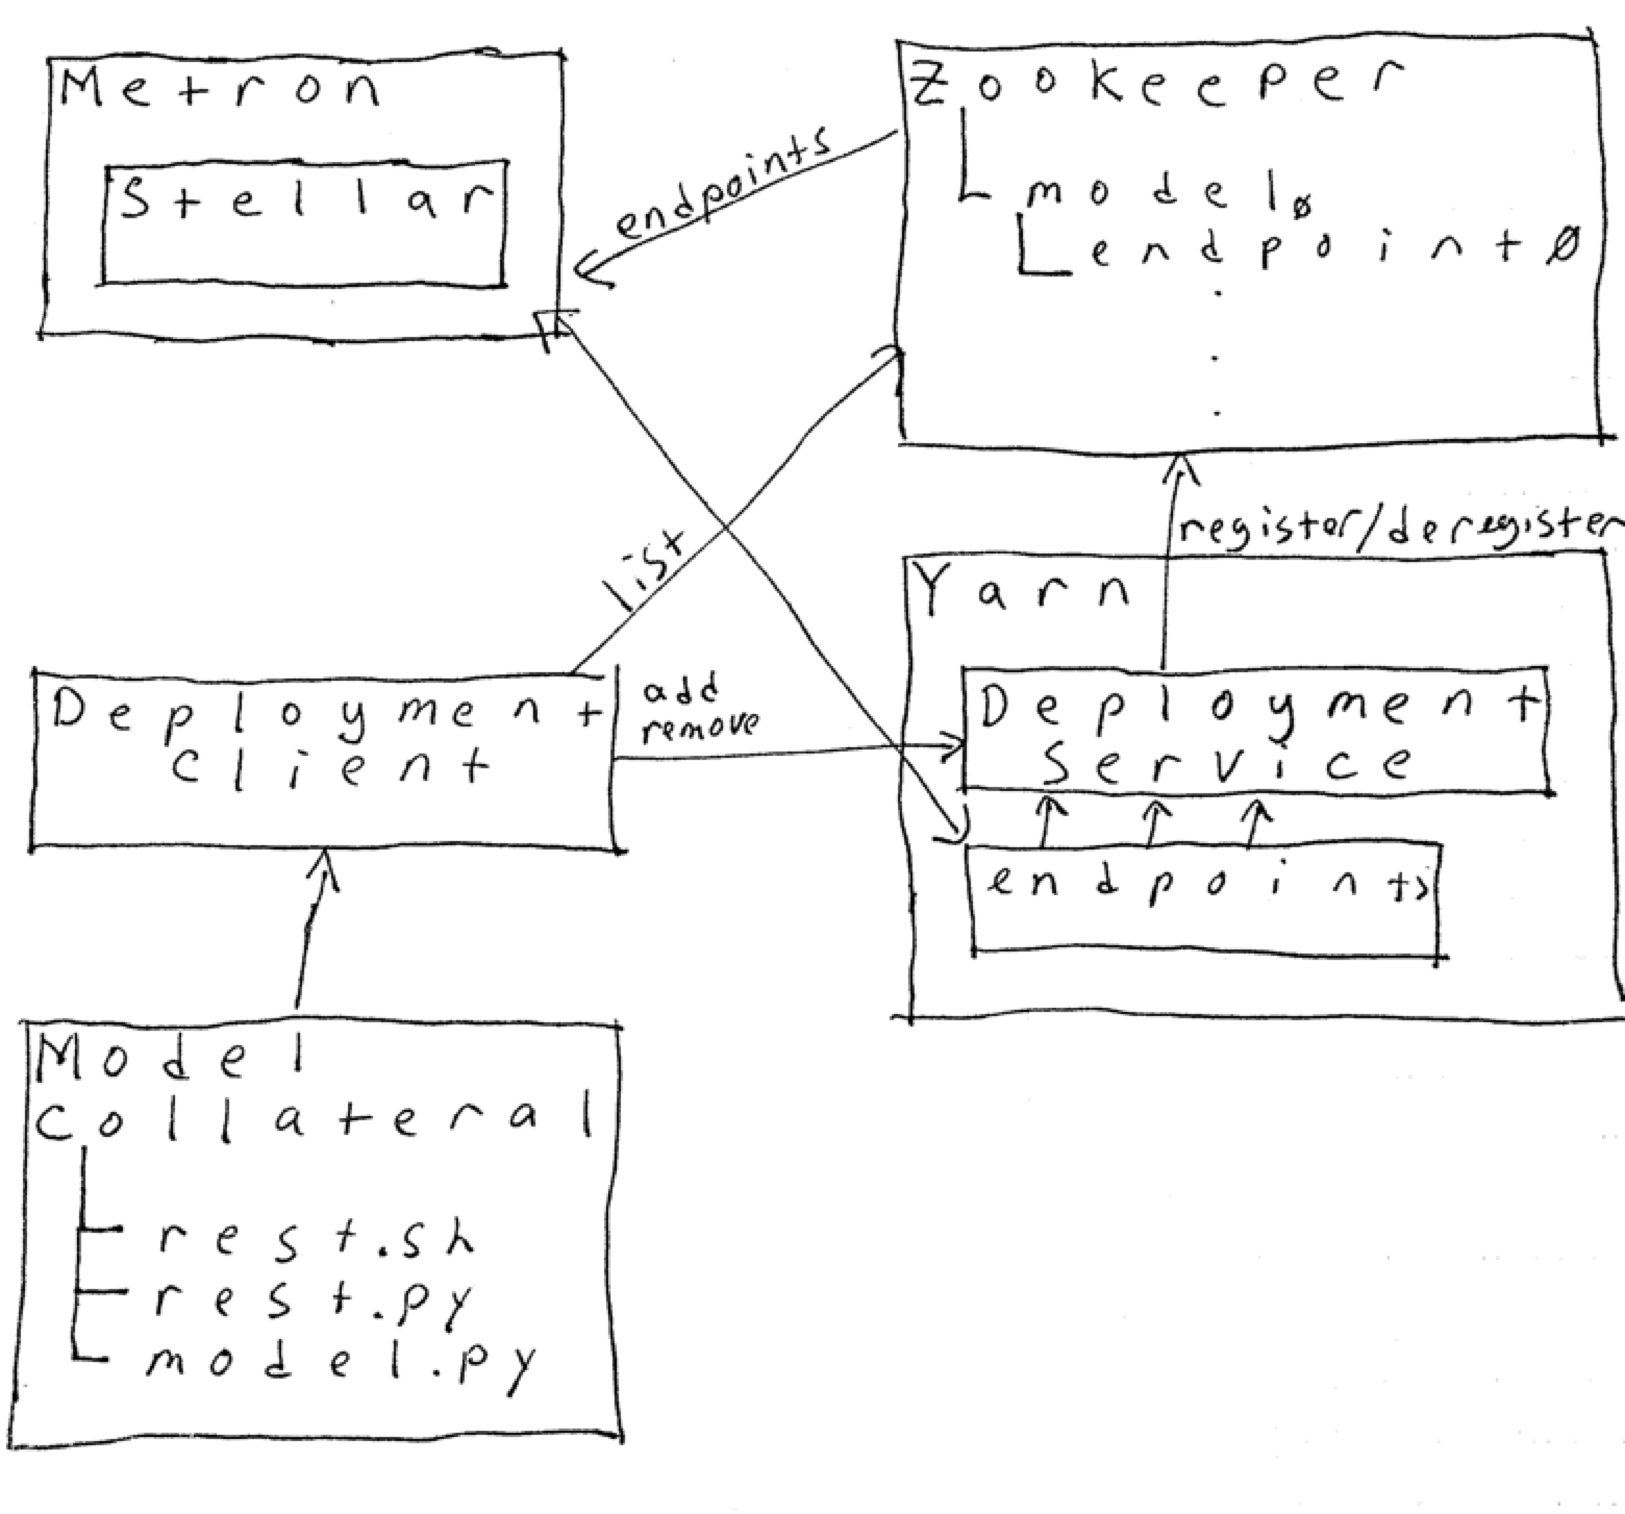
\includegraphics[scale=0.25]{images/maas_arch.png}}
\end{center}

}

\section{Domain Generating Algorithms}

\frame{\frametitle{Interlude: Domain Generating Algorithms}
Domain Generating Algorithms are used by botnets to communicate with compromised computers in an evasive way.
Traffic to a fixed command and control host would be noticed and firewall rules could be modified to cut communication channels cleanly.  
Instead, the botnet command and control hosts must move around to evade detection.  
Typically this involves periodically generating a synthetic domain in a repeatable way and having the compromised computers attempt to connect to a few candidate synthetic domains daily with some moderate hope of guessing the right one.  
This traffic is small enough to be lost in the shuffle of a large organization, making the evasion effective.
}

\frame{\frametitle{Demo}
\begin{itemize}
\item One solution for detecting synthetic domains is to construct a classifier that must be run against every domain going across the network.
\item At the BSides DFW Conference in 2013,  ClickSecurity presented a model written in Python for detecting synthetic domains.
\item We can expose this model as a REST endpoint, deploy via MaaS and interact with the model via Stellar
\end{itemize}
}

\section{Questions}

\frame{\frametitle{Questions}
Thanks for your attention!  Questions? 
\begin{itemize}
\item Find me at http://caseystella.com 
\item Twitter handle: @casey\_stella 
\item Email address: cstella@hortonworks.com
\end{itemize}
}

\end{document}
